\documentclass{article}

\usepackage{amssymb,amsmath,amsfonts,amsthm,epsfig}
\usepackage{dsfont}
\usepackage{algorithm}
\usepackage{url}
\usepackage{hhline}
\usepackage{setspace}
\usepackage{color}
\usepackage{fancyvrb}

%\usepackage{listings}
%\usepackage{fancybox}
%\usepackage{xcolor}


\usepackage{listings}
\usepackage{color}
\usepackage{textcomp}
\definecolor{listinggray}{gray}{0.9}
\definecolor{lbcolor}{rgb}{0.9,0.9,0.9}
\lstset{
	backgroundcolor=\color{lbcolor},
	tabsize=4,
	rulecolor=,
	language=matlab,
        basicstyle=\scriptsize,
        upquote=true,
        aboveskip={1.5\baselineskip},
        columns=fixed,
        showstringspaces=false,
        extendedchars=true,
        breaklines=true,
        prebreak = \raisebox{0ex}[0ex][0ex]{\ensuremath{\hookleftarrow}},
        frame=single,
        showtabs=false,
        showspaces=false,
        showstringspaces=false,
        identifierstyle=\ttfamily,
        keywordstyle=\color[rgb]{0,0,1},
        commentstyle=\color[rgb]{0.133,0.545,0.133},
        stringstyle=\color[rgb]{0.627,0.126,0.941},
}


\newcommand{\matlabcolor}{blue}

\newcommand{\matvar}[1]{\textcolor{\matlabcolor}{\tt {#1}}}

%\lstnewenvironment{Matlab}[1]{\lstset{#1, \textcolor{\matlabcolor}, basicstyle=\scriptsize, frame=shadowbox, rulesepcolor=\color{gray}, captionpos=b, abovecaptionskip=3mm, xleftmargin=1cm}}{}

% Example definitions.
% --------------------
\def\defequal{\stackrel{\mbox{\footnotesize def}}{=}}
\newcommand{\ve}[1]{ {\mathbf{#1}} }
\newcommand{\m}{\boldsymbol{\mu}}
\newcommand{\Sig}{\boldsymbol{\Sigma}}
\newcommand{\Lam}{\boldsymbol{\Lambda}}
\newcommand{\cequal}{\stackrel{\mbox{\footnotesize c}}{=}}
\newcommand{\btheta}{\boldsymbol{\theta}}
\newcommand{\balpha}{\boldsymbol{\alpha}}
%\newcommand{\diag}[1]{\mbox{diag}\left(#1\right)}
\newcommand{\trace}[1]{\mbox{trace}\left(#1\right)}
\def\EE{{\mathbb E}}
\def\diag{\mbox{diag}}
%\newcommand{\modif}[1]{\textbf{#1}}

\topmargin -1 cm
\textheight 23 cm
\oddsidemargin 0.7 cm
\textwidth 15 cm

%\doublespacing
\onehalfspacing

\begin{document}

\title{Flexible Audio Source Separation Toolbox (FASST) \\ Version 1.0 \\ User Guide}

\author{Alexey~Ozerov$~^1$, Emmanuel Vincent$~^1$ and Fr{\'e}d{\'e}ric Bimbot$~^2$ \\ \\
        $^1$INRIA, Centre de Rennes - Bretagne Atlantique \\
        $^2$ IRISA, CNRS - UMR 6074 \\
        Campus de Beaulieu, 35042 Rennes cedex, France\\
        {\tt\small \{alexey.ozerov, emmanuel.vincent\}@inria.fr, frederic.bimbot@irisa.fr} \\ \\}
\date{April 7, 2011}

\maketitle


\section{Introduction}

This user guide describes how to use FASST, an implementation of the general flexible source separation framework presented in \cite{Ozerov2010a}.
Before reading the user guide you are strongly encouraged to read \cite{Ozerov2010a}, at least the two first sections.

This guide is organized as follows. Some notations and abbreviations used throughout this document are listed in section~\ref{Sec_NotationsAbbrev}. Section~\ref{Sec_MixStruct} gives a detailed specification of the {\it mixture structure} (a Matlab structure), used to define the available prior information. The main functions the user should know about are listed in section~\ref{Sec_MainFunc} and an example of usage is given in section~\ref{Sec_UsageExample}.



\section{Some abbreviations and notations}
\label{Sec_NotationsAbbrev}


\subsection{Abbreviations}

\begin{tabular}{ll}
GMM    & Gaussian mixture model \\
GSMM   & Gaussian Scaled Mixture Model \\
HMM    & Hidden Markov Model \\
NMF    & Nonnegative matrix factorization \\
PSD    & Power Spectral Density \\
QERB   & Quadratic Equivalent Rectangular Bandwidth transform\\
S-HMM  & Scaled Hidden Markov Model \\
STFT   & Short-Time Fourier Transform \\
\end{tabular}


\subsection{Notations}

\begin{tabular}{ll}
$F$ & Number of frequency bins in the corresponding time-frequency representation \\

$N$ & Number of time frames in the corresponding time-frequency representation \\

$I$ & Number of channels (this version is only implemented for $I = 1$ or $I = 2$) \\

$J_{\rm spat}$ & Number of spatial components (see Section \ref{Sec_MixStruct})\\

$J_{\rm spec}$ & Number of spectral components (see Section \ref{Sec_MixStruct})\\
% (as compared to the description of the framework in \cite{Ozerov2010a}, \\
%& this implementation is more general in the sense that the number of spectral components \\ 
%& is not necessarily equal to that of spatial components, and more precisely $J_{\rm spec} \ge J_{\rm spat}$) \\

$R_j$ & Rank of the covariance matrix of the $j$-th spatial component  \\

$C_j$ & Number of factors in the $j$-th spectral component \\
      &  $-$ $C_j = 1$: direct model \\
      &  $-$ $C_j = 2$: factored excitation-filter model \\

$L^{\rm ex}_j$ & Number of narrowband excitation spectral patterns (see \cite{Ozerov2010a}) in the $j$-th spec. comp., \\

$K^{\rm ex}_j$ & Number of characteristic excitation spectral patterns (see \cite{Ozerov2010a}) in the $j$-th spec. comp., \\
%               & i.e., matrix ${\bf W}^{\rm ex}_j \cdot {\bf U}^{\rm ex}_j$ (see \cite{Ozerov2010a}) is of size $F \times K^{\rm ex}_j$ \\

$M^{\rm ex}_j$ & Number of time-localized excitation patterns (see \cite{Ozerov2010a}) in the $j$-th spec. comp., \\

$L^{\rm ft}_j$ & Number of narrowband filter spectral patterns (see \cite{Ozerov2010a}) in the $j$-th spec. comp., \\

$K^{\rm ft}_j$ & Number of characteristic filter spectral patterns (see \cite{Ozerov2010a}) in the $j$-th spec. comp., \\
%               & i.e., matrix ${\bf W}^{\rm ex}_j \cdot {\bf U}^{\rm ex}_j$ (see \cite{Ozerov2010a}) is of size $F \times K^{\rm ex}_j$ \\

$M^{\rm ft}_j$ & Number of time-localized filter patterns (see \cite{Ozerov2010a}) in the $j$-th spec. comp., \\

${\bf A}_j$ & Mixing parameters ($\in \mathbb C^{I \times R_j \times F \times N}$) in the $j$-th spatial comp. (see \cite{Ozerov2010a}), \\

${\bf W}^{\rm ex}_j$ & Narrowband excitation spectral patterns ($\in \mathbb R_+^{F \times L^{\rm ex}_j}$) in the $j$-th spec. comp. (see \cite{Ozerov2010a}), \\

${\bf U}^{\rm ex}_j$ & Excitation spectral pattern weights ($\in \mathbb R_+^{L^{\rm ex}_j \times K^{\rm ex}_j}$) in the $j$-th spec. comp. (see \cite{Ozerov2010a}), \\

${\bf G}^{\rm ex}_j$ & Excitation time pattern weights ($\in \mathbb R_+^{K^{\rm ex}_j \times M^{\rm ex}_j}$) in the $j$-th spec. comp. (see \cite{Ozerov2010a}), \\

${\bf H}^{\rm ex}_j$ & Time-localized excitation patterns ($\in \mathbb R_+^{M^{\rm ex}_j \times N}$) in the $j$-th spec. comp. (see \cite{Ozerov2010a}), \\

${\bf W}^{\rm ft}_j$ & Narrowband filter spectral patterns ($\in \mathbb R_+^{F \times L^{\rm ft}_j}$) in the $j$-th spec. comp. (see \cite{Ozerov2010a}), \\

${\bf U}^{\rm ft}_j$ & Filter spectral pattern weights ($\in \mathbb R_+^{L^{\rm ft}_j \times K^{\rm ft}_j}$) in the $j$-th spec. comp. (see \cite{Ozerov2010a}), \\

${\bf G}^{\rm ft}_j$ & Filter time pattern weights ($\in \mathbb R_+^{K^{\rm ft}_j \times M^{\rm ft}_j}$) in the $j$-th spec. comp. (see \cite{Ozerov2010a}), \\

${\bf H}^{\rm ft}_j$ & Time-localized filter patterns ($\in \mathbb R_+^{M^{\rm ft}_j \times N}$) in the $j$-th spec. comp. (see \cite{Ozerov2010a}), \\

$\mathbb R$ & Set of real numbers \\

$\mathbb R_+$ & Set of nonnegative real numbers \\

$\mathbb C$ & Set of complex numbers \\
\end{tabular}


\section{Mixture structure}
\label{Sec_MixStruct}

The mixture structure is a Matlab structure that is used to incorporate prior information into the framework.
The structure has a hierarchical organization that can be seen from the example in figure~\ref{Fig_MixStruct}.
Global parameters (e.g., signal representation) are defined on the first level of the hierarchy.
The second level consists of $J_{\rm spat}$ spatial components and $J_{\rm spec}$ spectral components.
Each source is typically modeled by one spectral component, although some sources (e.g., drums) might be modeled by several spectral components (e.g., bass drum, snare, etc.). Furthermore, each spectral component must be associated with one spatial component, and each spatial component
must have at least one spectral component associated to it.~\footnote{This extension makes it possible to model the fact that several sources have the same direction, which is very often the case for professionally produced music recordings. It is implemented by simply adding the power spectrograms of the spectral components corresponding to the same spatial component.}
Compared to the description of the framework in \cite{Ozerov2010a},
this implementation is more general in the sense that the number of spectral components
is not necessarily equal to that of spatial components, and more precisely $J_{\rm spec} \ge J_{\rm spat}$.
%Note that, as compared to the description of the framework in \cite{Ozerov2010a},
%this implementation is more general in the sense that the number of spectral components
%is not necessarily equal to that of spatial components, and more precisely $J_{\rm spec} \ge J_{\rm spat}$.
%Moreover, each spectral component must be associated with one spatial component, and each spatial component
%must have at least one spectral component associated to it.~\footnote{This extension makes it possible to model the fact that several sources have the same direction, which is very often the case for professionally produced music recordings. It is implemented by simply adding the power spectrograms of the spectral components corresponding to the same spatial component.}
The third level of the hierarchy consists in factorizing each spectral component into one or more {\it factors}
representing for instance excitation and filter structures 
(see \cite{Ozerov2010a})~\footnote{Note that in \cite{Ozerov2010a} the usage of two factors (excitation and filter) is described.
The implementation presented here is more flexible, since one can use any number of factors $C_j$, and it reduces to \cite{Ozerov2010a} when $C_j = 2$.
This is done for convenience of usage.
For example if one needs to implement an excitation model only or a filter model only ({\it direct model}), one simply needs to choose $C_j = 1$ without bothering to specify and to process an additional dummy factor.}.
Finally, on the fourth level of the hierarchy, each factor is represented as the product of three or four matrices
(see Table~\ref{Tab_Specfactor}), which are not represented in Figure~\ref{Fig_MixStruct}.
For instance, the factor representing excitation structure is either represented as the product of four matrices  ${\bf W}^{\rm ex}_j {\bf U}^{\rm ex}_j {\bf G}^{\rm ex}_j {\bf H}^{\rm ex}_j$ representing, respectively, narrowband spectral patterns, spectral pattern weights, time pattern weights and time-localized patterns (see \cite{Ozerov2010a}) or as the product of threes matrices  ${\bf W}^{\rm ex}_j {\bf U}^{\rm ex}_j {\bf G}^{\rm ex}_j$ when ${\bf H}^{\rm ex}_j$ is marked by the empty matrix \matvar{[]}~\footnote{In \cite{Ozerov2010a} only the case of four matrices is considered, and the case of three matrices ${\bf W}^{\rm ex}_j {\bf U}^{\rm ex}_j {\bf G}^{\rm ex}_j$ is just equivalent to fixing ${\bf H}^{\rm ex}_j$ to the $N \times N$ identity matrix. Since $N$ may be quite big, we fix ${\bf H}^{\rm ex}_j$ to \matvar{[]} by convention in the latter case in order to avoid storing a big identity matrix in memory.}.
Almost all the fields of the mixture structure must be filled as specified in Tables 
\ref{Tab_Mix_Str}, \ref{Tab_Spat_Comp}, \ref{Tab_Spec_Comp} and \ref{Tab_Specfactor}, except those marked by the empty matrix \matvar{[]}.

\begin{figure}[htbp]
%\begin{figure}[t]
%\begin{figure}[b]
  \begin{center}
    \leavevmode
%    \includegraphics[width=\columnwidth]{FlexFrame_in_a_nutshell}
    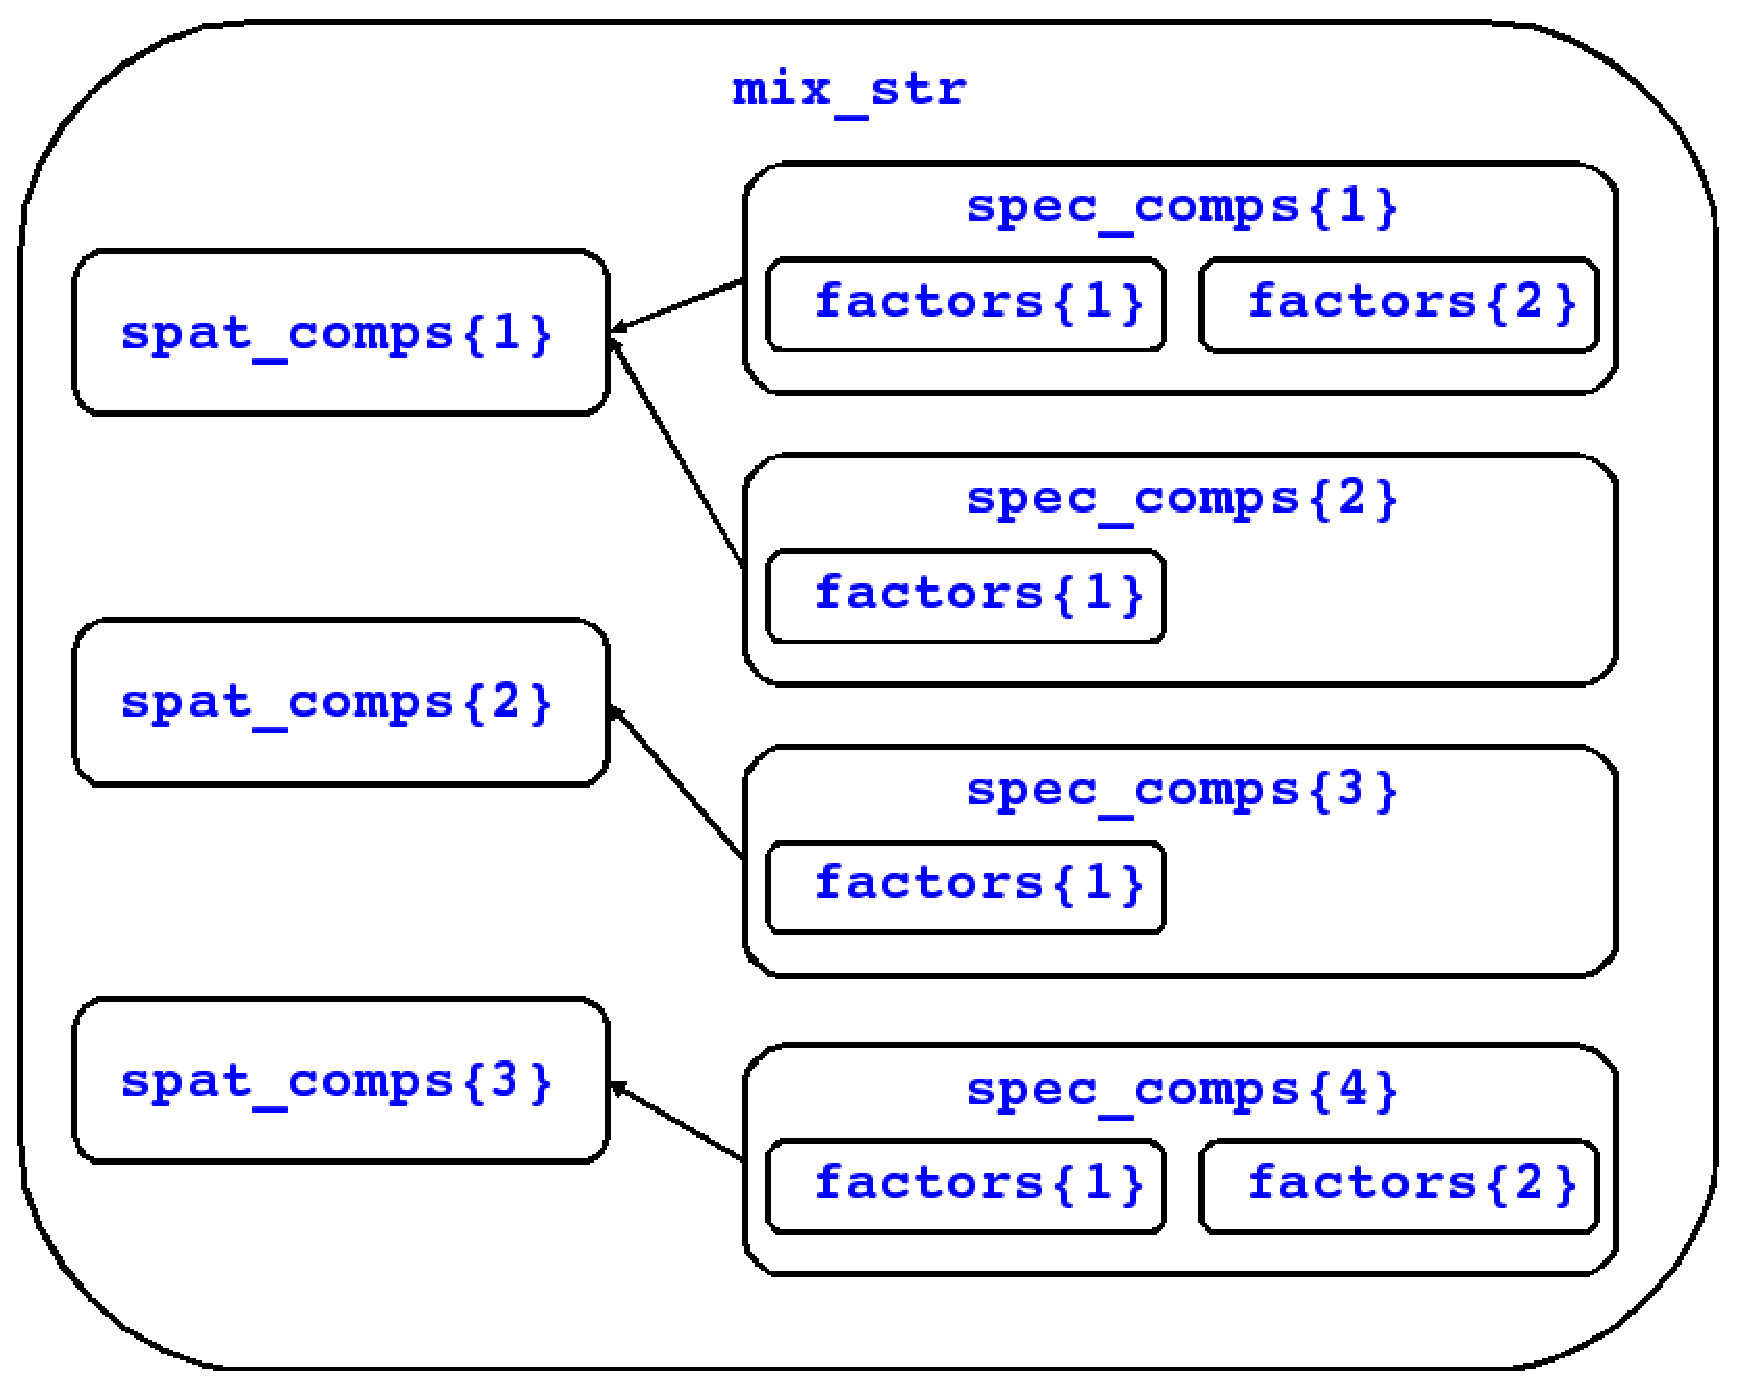
\includegraphics[width=12cm]{MixStruct_Ex}
    \caption{Visualization of a mixture structure example.}
    \label{Fig_MixStruct}
  \end{center}
\end{figure}

\section{Main functions}
\label{Sec_MainFunc}

The user should know about three main functions \matvar{comp\_transf\_Cx}, \matvar{estim\_param\_a\_post\_model} and \matvar{separate\_spec\_comps}, allowing, respectively, to compute the input time-frequency transform, estimate the model parameters and separate the spectral components. The headers of these functions are listed in Figures \ref{Tab_FuncCompTransf}, \ref{Tab_FuncParamEst} and \ref{Tab_SrcSep}.

\section{Examples of usage}
\label{Sec_UsageExample}

The user should also know how to fill and browse the mixture structure and how to use the above-mentioned three functions.
An example of mixture structure filling and browsing is given in Figures \ref{Tab_MixStructFillingExample} and \ref{Tab_MixStrBowsing}.
%shows browsing in Matlab of a structure obtained with this example.
An example script
%using functions \matvar{comp\_transf\_Cx}, \matvar{estim\_param\_a\_post\_model} and \matvar{separate\_spec\_comps} to separate 
for the separation of an instantaneous mixture of music signals is given in Figure \ref{Tab_UsageExamp}.

Function \matvar{EXAMPLE\_prof\_rec\_sep\_drums\_bass\_melody.m} contains a more sophisticated example allowing the separation of the following four sources:
\begin{itemize}
\item drums,
\item bass,
\item melody (singing voice or leading melodic instrument),
\item remaining sounds,
\end{itemize}
from a stereo music recording.
Due to memory limits in Matlab this function cannot process sound excerpts longer than 30 seconds.
For full length music recording the function \\
\matvar{EXAMPLE\_prof\_rec\_sep\_drums\_bass\_melody\_FULL.m} \\
should be used.
This function simply cuts the full recording into small parts, and applies \\
\matvar{EXAMPLE\_prof\_rec\_sep\_drums\_bass\_melody.m} to each of them.


\bibliographystyle{IEEEtran}
\bibliography{FASST_UserGuide_v1}

\newpage

%\begin{figure}[htbp]
\begin{table}[t]
  \begin{center}
%    \arrayrulewidth=0.1em
%   \scriptsize 
   \begin{tabular}{l|l|l}
      Field & Description & Value \\
      \hhline{===}
       \matvar{Cx} & $F \times N \times I \times I$ complex-valued tensor of local & \raisebox{-4.5pt}[0pt][0pt]{$\in \mathbb C^{F \times N \times I \times I}$} \\
                & mixture covariances & \\
      \hhline{---}
       \matvar{transf} & Input time-frequency transform & \matvar{'stft'} for STFT \\
      \hhline{~~-}
                    &           & \matvar{'qerb'} for QERB \\
      \hhline{---}
       \matvar{fs} & Sampling frequency in Hz & $\in \{ 16000, 44100, \ldots \}$ \\
      \hhline{---}
       \matvar{wlen} & Analysis window length & $\in \{ 512, 1024, \ldots \}$ \\
                  & (used to compute STFT or QERB) in samples & \\
      \hhline{---}
       \matvar{Noise\_PSD} & $F \times 1$ real-valued nonnegative vector of additive & \raisebox{-4.5pt}[0pt][0pt]{$\in \mathbb R^{1 \times F}$ or \matvar{[]}} \\
                        & noise PSD, e.g., for annealing &  \\
      \hhline{---}
       \matvar{spat\_comps} & $1 \times J_{\rm spat}$ cell array of spatial component structures & see Table~\ref{Tab_Spat_Comp} \\
      \hhline{---}
       \matvar{spec\_comps} & $1 \times J_{\rm spec}$ cell array of spectral component structures & see Table~\ref{Tab_Spec_Comp} \\
      \hhline{===}
    \end{tabular}
    \caption{Specification of the mixture structure (\matvar{mix\_str}).}
    \label{Tab_Mix_Str}
  \end{center}
\end{table}

%\begin{figure}[htbp]
\begin{table}[t]
  \begin{center}
%    \arrayrulewidth=0.1em
%   \scriptsize 
   \begin{tabular}{l|l|l}
      Field & Description & Value \\
      \hhline{===}
       \matvar{time\_dep} & Stationarity of mixing & \matvar{'indep'} for time-invariant mixing \\
      \hhline{~~-}
                       &                             & \matvar{'dep'} for time-varying mixing \\
      \hhline{---}
       \matvar{mix\_type} & Mixing type & \matvar{'inst'} for instantaneous (freq.-indep.) \\
      \hhline{~~-}
                       &             & \matvar{'conv'} for convolutive (freq.-dep.) \\
      \hhline{---}
       \matvar{frdm\_prior} & Degree of adaptability & \matvar{'free'} for adaptive \\
      \hhline{~~-}
                         &                        & \matvar{'fixed'} for fixed  \\
      \hhline{---}
       \matvar{params} & Tensor of mixing parameters & \raisebox{-1.5pt}[0pt][0pt]{$\in \mathbb R^{I \times R_j}$} $\quad$ for \matvar{mix\_type = 'inst'}\\
      \hhline{~~-}
                    & (corresponding to ${\bf A}_j$ from \cite{Ozerov2010a}) & \raisebox{-1.5pt}[0pt][0pt]{$\in \mathbb C^{I \times R_j \times F}$} $\quad$ for \matvar{mix\_type = 'conv'} \\
      \hhline{===}
    \end{tabular}
    \caption{Specification of the spatial component structure (\matvar{spat\_comps\{j\}}, $j = 1, \ldots, J_{\rm spat}$).}
    \label{Tab_Spat_Comp}
  \end{center}
\end{table}

%\begin{figure}[htbp]
\begin{table}[t]
  \begin{center}
%    \arrayrulewidth=0.1em
%   \scriptsize 
   \begin{tabular}{l|l|l}
      Field & Description & Value \\
      \hhline{===}
       \matvar{spat\_comp\_ind} & Index of the corresponding spatial component &  $\in \{1, \ldots, J_{\rm spat} \}$ \\
      \hhline{---}
       \matvar{factors} & $1 \times L_j$ cell array of factor structures & \\
      \hhline{===}
    \end{tabular}
    \caption{Specification of the spectral component structure (\matvar{spec\_comps\{j\}}, $j = 1, \ldots, J_{\rm spec}$).}
    \label{Tab_Spec_Comp}
  \end{center}
\end{table}

%\begin{figure}[htbp]
\begin{table}[t]
  \begin{center}
%    \arrayrulewidth=0.1em
%   \scriptsize 
   \begin{tabular}{l|l|l}
      Field & Description & Value \\
      \hhline{===}
       \matvar{FB\_frdm\_prior} & Degree of adaptability & \matvar{'free'} for adaptive \\
      \hhline{~~-}
                       & for narrowband spectral patterns & \matvar{'fixed'} for fixed \\
      \hhline{---}
       \matvar{FW\_frdm\_prior} & Degree of adaptability & \matvar{'free'} for adaptive \\
      \hhline{~~-}
                       & for spectral pattern weights & \matvar{'fixed'} for fixed \\
      \hhline{---}
       \matvar{TW\_frdm\_prior} & Degree of adaptability & \matvar{'free'} for adaptive \\
      \hhline{~~-}
                       & for time pattern weights & \matvar{'fixed'} for fixed \\
      \hhline{---}
       \matvar{TB\_frdm\_prior} & Degree of adaptability & \matvar{'free'} for adaptive \\
      \hhline{~~-}
                       & for time-localized patterns & \matvar{'fixed'} for fixed \\
      \hhline{---}
       \matvar{FB} & Narrowband spectral patterns (Frequency Blobs) & \raisebox{-5.5pt}[0pt][0pt]{$\in \mathbb R_+^{F \times L^{\rm ex}_j}$ or $\in \mathbb R_+^{F \times L^{\rm ft}_j}$} \\
                   & (corresponding to ${\bf W}^{\rm ex}_j$ or ${\bf W}^{\rm ft}_j$) &  \\
      \hhline{---}
       \matvar{FW} & Spectral pattern weights (Frequency Weights) & \raisebox{-5.5pt}[0pt][0pt]{$\in \mathbb R_+^{L^{\rm ex}_j \times K^{\rm ex}_j}$ or $\in \mathbb R_+^{L^{\rm ft}_j \times K^{\rm ft}_j}$} \\
                   & (corresponding to ${\bf U}^{\rm ex}_j$ or ${\bf U}^{\rm ft}_j$) &  \\
      \hhline{---}
       \matvar{TW} & Time pattern weights (Time Weights) & \raisebox{-5.5pt}[0pt][0pt]{$\in \mathbb R_+^{K^{\rm ex}_j \times M^{\rm ex}_j}$ or $\in \mathbb R_+^{K^{\rm ft}_j \times M^{\rm ft}_j}$} \\
                   & (corresponding to ${\bf G}^{\rm ex}_j$ or ${\bf G}^{\rm ft}_j$) &  \\
      \hhline{---}
       \matvar{TB} & Time-localized patterns (Time Blobs) & \raisebox{-5.5pt}[0pt][0pt]{$\in \mathbb R_+^{M^{\rm ex}_j \times N}$, $\in \mathbb R_+^{M^{\rm ft}_j \times N}$ or \matvar{[]}} \\
                   & (corresponding to ${\bf H}^{\rm ex}_j$ or ${\bf H}^{\rm ft}_j$) &  \\
      \hhline{---}
       \matvar{TW\_constr} & Constraint on the time pattern weights & \matvar{'NMF'} no constraint \\
      \hhline{~~-}
                       & (note that nontrivial constraints, i.e.,   & \matvar{'GMM'} for GMM \\
      \hhline{~~-}
                       & different from \matvar{'NMF'} are not      & \matvar{'HMM'} for HMM \\
      \hhline{~~-}
                       & compatible with nonempty time patterns \matvar{TB})  & \matvar{'GSMM'} for GSMM \\
      \hhline{~~-}
                       &                                      & \matvar{'SHMM'} for S-HMM \\
      \hhline{---}
       \matvar{TW\_DP\_params} & Discrete probability (DP) parameters & $1 \times K^{\rm ex}_j$ ($1 \times K^{\rm ft}_j$) vector \\
                               & for the time pattern weights                              & of Gaussian weights                             \\
                               & (needed only when \matvar{TW\_constr} $\ne$ \matvar{'NMF'})  & for GMM or GSMM                              \\
      \hhline{~~-}
                       &                                                           & $K^{\rm ex}_j \times K^{\rm ex}_j$ ($K^{\rm ft}_j \times K^{\rm ft}_j$) \\
                       &                                                           & matrix of transition\\
                               &                                                   &  probabilities                    \\
                               &                                                   & for HMM or S-HMM                              \\
      \hhline{---}
       \matvar{TW\_DP\_frdm\_prior} & Degree of adaptability for DP parameters & \matvar{'free'} for adaptive \\
      \hhline{~~-}
                       & (needed only when \matvar{TW\_constr} $\ne$ \matvar{'NMF'}) & \matvar{'fixed'} for fixed \\
      \hhline{---}
       \matvar{TW\_all} & Matrix of all time weights & Nonnegative real-valued \\
                       & (corresponding to ${\bf \tilde G}^{\rm ex}_j$ or ${\bf \tilde G}^{\rm ft}_j$ from \cite{Ozerov2010a}) & matrix of the same  \\
                       & (needed only when \matvar{TW\_constr} $\ne$ \matvar{'NMF'}) & size as \matvar{TW} \\
      \hhline{===}
    \end{tabular}
    \caption{Specification of the spectral component factor structure (\matvar{factors\{l\}}, $l = 1, \ldots, L_j$).
     % Note that matrices \matvar{FB}, \matvar{FW}, \matvar{TW} and \matvar{TB} must be so that either \matvar{FB * FW * TW * TB} or \matvar{FB * FW * TW} (if \matvar{TB} is an empty matrix) is of size $F \times N$.
     }
    \label{Tab_Specfactor}
  \end{center}
\end{table}



%\begin{figure}[htbp]
\begin{figure}[t]
\begin{center}
	\begin{lstlisting}
function Cx = comp_transf_Cx(x, transf, win_len, fs, qerb_nbin)

%
% Cx = comp_transf_Cx(x, transf, win_len, fs, qerb_nbin);
%
% compute spatial covariance matrices for the corresponding transform
%
%
% input 
% -----
%
% x                 : [I x nsampl] matrix containing I time-domain mixture signals
%                     with nsampl samples
% transf            : transform
%                       'stft'
%                       'qerb'
% win_len           : window length
% fs                : (opt) sampling frequency (Hz)
% qerb_nbin         : (opt) number of bins for qerb transform
%
% output
% ------
%
% Cx                : [F x N x I x I] matrix containing the spatial covariance
%                     matrices of the input signal in all time-frequency bins
%
	\end{lstlisting}
    \caption{\matvar{comp\_transf\_Cx} : FASST function for the computation of the input time-frequency transform.}
    \label{Tab_FuncCompTransf}
\end{center}
\end{figure}


%\begin{figure}[htbp]
\begin{figure}[t]
\begin{center}
	\begin{lstlisting}
function [mix_str, log_like_arr] = estim_param_a_post_model(mix_str_inp, ...
    iter_num, sim_ann_opt, Ann_PSD_beg, Ann_PSD_end)

%
% [mix_str, log_like_arr] = estim_param_a_post_model(mix_str_inp, ...
%    iter_num, sim_ann_opt, Ann_PSD_beg, Ann_PSD_end);
%
% estimate a posteriori mixture model parameters
%
%
% input
% -----
%
% mix_str_inp       : input mixture structure
% iter_num          : (opt) number of EM iterations (def = 100)
% sim_ann_opt       : (opt) simulated annealing option (def = 'ann')
%                        'no_ann'     : no annealing (zero noise)
%                        'ann'        : annealing
%                        'ann_ns_inj' : annealing with noise injection
%                        'upd_ns_prm' : update noise parameters
%                                       (Noise_PSD is updated through EM)
% Ann_PSD_beg       : (opt) [F x 1] beginning vector of annealing noise PSD
%                           (def = X_power / 100)
% Ann_PSD_end       : (opt) [F x 1] end vector of annealing noise PSD
%                           (def = X_power / 10000)
% 
%
% output
% ------
%
% mix_str           : estimated output mixture structure
% log_like_arr      : array of log-likelihoods
%
	\end{lstlisting}
    \caption{\matvar{estim\_param\_a\_post\_model} : FASST function for the estimation of the model parameters.}
    \label{Tab_FuncParamEst}
\end{center}
\end{figure}


%\begin{figure}[htbp]
\begin{figure}[t]
\begin{center}
	\begin{lstlisting}
function ie = separate_spec_comps(x, mix_str, sep_cmp_inds)

%
% ie = separate_spec_comps(x, mix_str, sep_cmp_inds);
%
% separate spectral components
%
%
% input
% -----
%
% x                 : [nchan x nsampl] mixture signal
% mix_str           : input mix structure
% sep_cmp_inds      : (opt) array of indices for components to separate
%                     (def = {1, 2, ..., K_spec})
% 
%
% output
% ------
%
% ie                : [K_sep x nsampl x nchan] estimated spectral components images,
%                     where K_sep = length(sep_cmp_inds) is the number of
%                     components to separate
%
	\end{lstlisting}
    \caption{\matvar{separate\_spec\_comps} : FASST function for the separation of the spectral component signals.}
    \label{Tab_SrcSep}
\end{center}
\end{figure}




%\begin{figure}[htbp]
\begin{figure}[t]
\begin{center}
	\lstinputlisting{../init_mix_struct_Mult_NMF_inst.m}
    \caption{Example of filling of the mixture structure corresponding to the multichannel NMF method \cite{Ozerov2009b} (instantaneous case).}
    \label{Tab_MixStructFillingExample}
\end{center}
\end{figure}

%\begin{figure}[htbp]
\begin{figure}[t]
\begin{center}
	\begin{lstlisting}
>> mix_str

mix_str = 

            Cx: [4-D double]
        transf: 'stft'
            fs: 16000
          wlen: 1024
    spat_comps: {[1x1 struct]  [1x1 struct]  [1x1 struct]}
    spec_comps: {[1x1 struct]  [1x1 struct]  [1x1 struct]}
     Noise_PSD: [513x1 double]

>> mix_str.spat_comps{2}

ans = 

      time_dep: 'indep'
      mix_type: 'inst'
    frdm_prior: 'free'
        params: [2x1 double]

>> mix_str.spec_comps{3}

ans = 

    spat_comp_ind: 3
          factors: {[1x1 struct]}

>> mix_str.spec_comps{3}.factors{1}

ans = 

               FB: [513x4 double]
               FW: [4x4 double]
               TW: [4x98 double]
               TB: []
    FB_frdm_prior: 'free'
    FW_frdm_prior: 'fixed'
    TW_frdm_prior: 'free'
    TB_frdm_prior: []
        TW_constr: 'NMF'
	\end{lstlisting}
    \caption{Browsing in Matlab of the example mixture structure in Table \ref{Tab_MixStructFillingExample}.}
    \label{Tab_MixStrBowsing}
\end{center}
\end{figure}


%\begin{figure}[htbp]
\begin{figure}[t]
\begin{center}
	\lstinputlisting{../EXAMPLE_ssep_Mult_NMF_inst.m}
    \caption{Example of usage involving all three main functions (runs the multichannel NMF method \cite{Ozerov2009b} in the instantaneous case).}
    \label{Tab_UsageExamp}
\end{center}
\end{figure}




\end{document}
